\section{Design}
\label{sec:design}

The design mainline are composed of ``Market Strategy'', ``System and Process'', and ``User Interface and Interaction'' to separate the business matters, logic elements, and display view.

% --------------------------------------------------
\subsection{Target User}

For our target user, strategy we're using is actually kind of concise. In the business related segment, it is by using what we call a \ac{BMC}\index{Business Model Canvas} to help shape the product which users would use up to customers would pay for. More details on this can be seen in \autoref{chap:theory}.
Also as concerns of a wide range of market, we're is not impartially refer to one of between the subject is a common vertical market (generally anyone, ordinary regular users and such) or diagonal market (specific types, from professionals to large industries).
Instead, we want to take a different approach.
We found and chose a what we came up with, a diagonal market which anyone can be a user and even a customer.
This could cover both vertical and diagonal market within the same product.
Diagonal product can be too risky if we don't have a focus.
So we first defined and validate the more likely to be considered which seems only be the users and customers.
The general ones are individuals, small teams, students, educators, teachers, managers, creatives, developers, designers. The specific ones are entrepreneurs, software and information architect, strategy consultants, research analysts, organization managers, data analysts, and even \ac{CTO}.
The culmination of this product is a general purpose type of tool that benefits both side of the worlds.
We can breakdown them each, later in the implementation chapter which also discuss the core features of what we're making.
But as explained in \autoref{sec:problem-scope}, we can't design for everyone in the beginning.
So we chose employees and colleagues in a startup work environment to be the initial focus.
Because we know what we design for, we can effectively start our design.

% --------------------------------------------------
\subsection{Application Architecture}

...
%Based on Simple Web App Architecture, inspired

\autoref{fig:satellid-arch-app}

\begin{figure}[htbp]
    \centering
    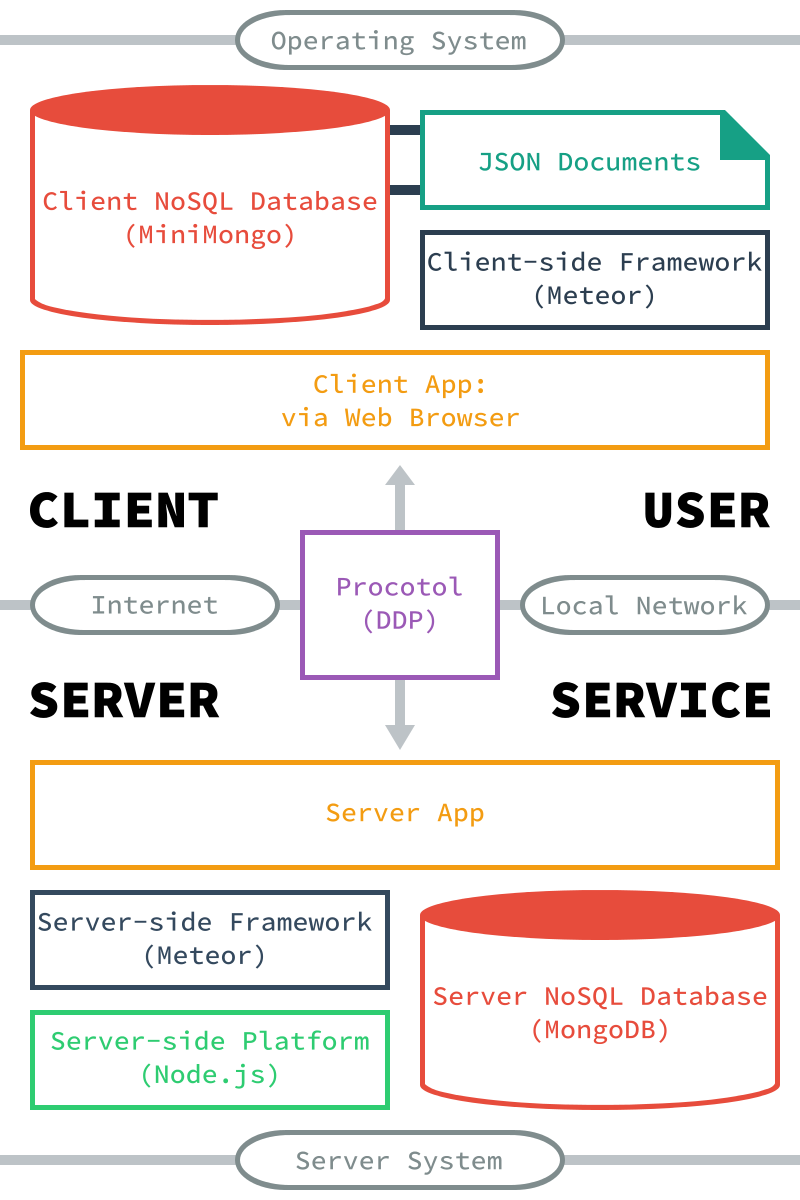
\includegraphics[width=8cm]{\dir/include/satellid-arch-app.png}
    \caption[Satellid Application Architecture]{The architecture of Satellid application}
    \label{fig:satellid-arch-app}
\end{figure}

% --------------------------------------------------
\subsection{System and Process}

In the product segment, it is by shortening the steps that needed to do a knowledge management, with making it more effective and accessible. Satellid uses an major role of features called ``Contextual'' and ``Superbar''.

\begin{figure}[htb]
    \centering
    % \includegraphics[width=\textwidth]{\dir/include/contextual}
    \caption{Contextual visual representation}
    \label{fig:background:contextual}
\end{figure}

Contextual utilize data and template that are used together to form the context and structure.
With this, user will eventually always structure their data, and even create more or modify available data field.
In addition to this, category and tagging could also be built.
At the later time, it can be easily sorted faster than just using category or tags.
The difference of context with category or tag is how it handles specificity.
Context is very specific as a descriptor so it can be fully understood and assessed easily, rather than category or tag that is more widely and freely determined.
For example, \textit{The Merriam-Webster Dictionary} may be categorized as a ``dictionary'', ``book'', ``reference'', ``glossary'', ``thesaurus'' and tagged as ``word'', ``language'', ``english'', ``''; but it is basically just a ``publication''.
So it can be in the same context like \text{JavaScript, The Definitive Guide} or even \text{Iron Man comic}.
Contextual provide some of the most common type of knowledge with its key attributes.
As a sample, the lists below are the sorted version of prospected key attributes that can be used.
Each of them can have a label if appropriate.

\begin{easylist}
& Basic
  && ID
  && Context
  && Date
     &&& Created
     &&& Updated
  && Time
  && Location
  && Content/Text
& Person
  && Name
  && Location
  && Phone
  && Email
& Organization
  && Name
  && Type
  && Industry
  && Founded
& Product
  && Name
  && Type
  && Tagline
  && Description
& Publication
  && Name
  && Author
  && Description
& Event
  && Title
  && Type
  && Location
  && Date
  && Presenter
\end{easylist}

Superbar enable \ac{CRUD} and search operation simultaneously within the same interaction interface box (the space or the bar).

\begin{figure}[htb]
    \centering
    % \includegraphics[width=\textwidth]{\dir/include/superbar}
    \caption{Superbar interface}
    \label{fig:background:superbar}
\end{figure}

% --------------------------------------------------
\subsection{User Interface and Interaction}

Here are some of the user interfaces on the web version of Satellid.

%TODO User flow

% --------------------------------------------------
\subsection{Data Schema Design}

%TODO Related to MongoDB
